
%% bare_conf.tex
%% V1.4b
%% 2015/08/26
%% by Michael Shell
%% See:
%% http://www.michaelshell.org/
%% for current contact information.
%%
%% This is a skeleton file demonstrating the use of IEEEtran.cls
%% (requires IEEEtran.cls version 1.8b or later) with an IEEE
%% conference paper.
%%
%% Support sites:
%% http://www.michaelshell.org/tex/ieeetran/
%% http://www.ctan.org/pkg/ieeetran
%% and
%% http://www.ieee.org/

%%*************************************************************************
%% Legal Notice:
%% This code is offered as-is without any warranty either expressed or
%% implied; without even the implied warranty of MERCHANTABILITY or
%% FITNESS FOR A PARTICULAR PURPOSE! 
%% User assumes all risk.
%% In no event shall the IEEE or any contributor to this code be liable for
%% any damages or losses, including, but not limited to, incidental,
%% consequential, or any other damages, resulting from the use or misuse
%% of any information contained here.
%%
%% All comments are the opinions of their respective authors and are not
%% necessarily endorsed by the IEEE.
%%
%% This work is distributed under the LaTeX Project Public License (LPPL)
%% ( http://www.latex-project.org/ ) version 1.3, and may be freely used,
%% distributed and modified. A copy of the LPPL, version 1.3, is included
%% in the base LaTeX documentation of all distributions of LaTeX released
%% 2003/12/01 or later.
%% Retain all contribution notices and credits.
%% ** Modified files should be clearly indicated as such, including  **
%% ** renaming them and changing author support contact information. **
%%*************************************************************************


% *** Authors should verify (and, if needed, correct) their LaTeX system  ***
% *** with the testflow diagnostic prior to trusting their LaTeX platform ***
% *** with production work. The IEEE's font choices and paper sizes can   ***
% *** trigger bugs that do not appear when using other class files.       ***                          ***
% The testflow support page is at:
% http://www.michaelshell.org/tex/testflow/



\documentclass[conference]{IEEEtran}
% Some Computer Society conferences also require the compsoc mode option,
% but others use the standard conference format.
%
% If IEEEtran.cls has not been installed into the LaTeX system files,
% manually specify the path to it like:
% \documentclass[conference]{../sty/IEEEtran}





% Some very useful LaTeX packages include:
% (uncomment the ones you want to load)


% *** MISC UTILITY PACKAGES ***
%
%\usepackage{ifpdf}
% Heiko Oberdiek's ifpdf.sty is very useful if you need conditional
% compilation based on whether the output is pdf or dvi.
% usage:
% \ifpdf
%   % pdf code
% \else
%   % dvi code
% \fi
% The latest version of ifpdf.sty can be obtained from:
% http://www.ctan.org/pkg/ifpdf
% Also, note that IEEEtran.cls V1.7 and later provides a builtin
% \ifCLASSINFOpdf conditional that works the same way.
% When switching from latex to pdflatex and vice-versa, the compiler may
% have to be run twice to clear warning/error messages.






% *** CITATION PACKAGES ***
%
%\usepackage{cite}
% cite.sty was written by Donald Arseneau
% V1.6 and later of IEEEtran pre-defines the format of the cite.sty package
% \cite{} output to follow that of the IEEE. Loading the cite package will
% result in citation numbers being automatically sorted and properly
% "compressed/ranged". e.g., [1], [9], [2], [7], [5], [6] without using
% cite.sty will become [1], [2], [5]--[7], [9] using cite.sty. cite.sty's
% \cite will automatically add leading space, if needed. Use cite.sty's
% noadjust option (cite.sty V3.8 and later) if you want to turn this off
% such as if a citation ever needs to be enclosed in parenthesis.
% cite.sty is already installed on most LaTeX systems. Be sure and use
% version 5.0 (2009-03-20) and later if using hyperref.sty.
% The latest version can be obtained at:
% http://www.ctan.org/pkg/cite
% The documentation is contained in the cite.sty file itself.

\usepackage{graphicx}
\usepackage{amsmath}




% *** GRAPHICS RELATED PACKAGES ***
%
\ifCLASSINFOpdf
  % \usepackage[pdftex]{graphicx}
  % declare the path(s) where your graphic files are
  % \graphicspath{{../pdf/}{../jpeg/}}
  % and their extensions so you won't have to specify these with
  % every instance of \includegraphics
  % \DeclareGraphicsExtensions{.pdf,.jpeg,.png}
\else
  % or other class option (dvipsone, dvipdf, if not using dvips). graphicx
  % will default to the driver specified in the system graphics.cfg if no
  % driver is specified.
  % \usepackage[dvips]{graphicx}
  % declare the path(s) where your graphic files are
  % \graphicspath{{../eps/}}
  % and their extensions so you won't have to specify these with
  % every instance of \includegraphics
  % \DeclareGraphicsExtensions{.eps}
\fi
% graphicx was written by David Carlisle and Sebastian Rahtz. It is
% required if you want graphics, photos, etc. graphicx.sty is already
% installed on most LaTeX systems. The latest version and documentation
% can be obtained at: 
% http://www.ctan.org/pkg/graphicx
% Another good source of documentation is "Using Imported Graphics in
% LaTeX2e" by Keith Reckdahl which can be found at:
% http://www.ctan.org/pkg/epslatex
%
% latex, and pdflatex in dvi mode, support graphics in encapsulated
% postscript (.eps) format. pdflatex in pdf mode supports graphics
% in .pdf, .jpeg, .png and .mps (metapost) formats. Users should ensure
% that all non-photo figures use a vector format (.eps, .pdf, .mps) and
% not a bitmapped formats (.jpeg, .png). The IEEE frowns on bitmapped formats
% which can result in "jaggedy"/blurry rendering of lines and letters as
% well as large increases in file sizes.
%
% You can find documentation about the pdfTeX application at:
% http://www.tug.org/applications/pdftex





% *** MATH PACKAGES ***
%
%\usepackage{amsmath}
% A popular package from the American Mathematical Society that provides
% many useful and powerful commands for dealing with mathematics.
%
% Note that the amsmath package sets \interdisplaylinepenalty to 10000
% thus preventing page breaks from occurring within multiline equations. Use:
%\interdisplaylinepenalty=2500
% after loading amsmath to restore such page breaks as IEEEtran.cls normally
% does. amsmath.sty is already installed on most LaTeX systems. The latest
% version and documentation can be obtained at:
% http://www.ctan.org/pkg/amsmath





% *** SPECIALIZED LIST PACKAGES ***
%
%\usepackage{algorithmic}
% algorithmic.sty was written by Peter Williams and Rogerio Brito.
% This package provides an algorithmic environment fo describing algorithms.
% You can use the algorithmic environment in-text or within a figure
% environment to provide for a floating algorithm. Do NOT use the algorithm
% floating environment provided by algorithm.sty (by the same authors) or
% algorithm2e.sty (by Christophe Fiorio) as the IEEE does not use dedicated
% algorithm float types and packages that provide these will not provide
% correct IEEE style captions. The latest version and documentation of
% algorithmic.sty can be obtained at:
% http://www.ctan.org/pkg/algorithms
% Also of interest may be the (relatively newer and more customizable)
% algorithmicx.sty package by Szasz Janos:
% http://www.ctan.org/pkg/algorithmicx




% *** ALIGNMENT PACKAGES ***
%
%\usepackage{array}
% Frank Mittelbach's and David Carlisle's array.sty patches and improves
% the standard LaTeX2e array and tabular environments to provide better
% appearance and additional user controls. As the default LaTeX2e table
% generation code is lacking to the point of almost being broken with
% respect to the quality of the end results, all users are strongly
% advised to use an enhanced (at the very least that provided by array.sty)
% set of table tools. array.sty is already installed on most systems. The
% latest version and documentation can be obtained at:
% http://www.ctan.org/pkg/array


% IEEEtran contains the IEEEeqnarray family of commands that can be used to
% generate multiline equations as well as matrices, tables, etc., of high
% quality.




% *** SUBFIGURE PACKAGES ***
%\ifCLASSOPTIONcompsoc
%  \usepackage[caption=false,font=normalsize,labelfont=sf,textfont=sf]{subfig}
%\else
%  \usepackage[caption=false,font=footnotesize]{subfig}
%\fi
% subfig.sty, written by Steven Douglas Cochran, is the modern replacement
% for subfigure.sty, the latter of which is no longer maintained and is
% incompatible with some LaTeX packages including fixltx2e. However,
% subfig.sty requires and automatically loads Axel Sommerfeldt's caption.sty
% which will override IEEEtran.cls' handling of captions and this will result
% in non-IEEE style figure/table captions. To prevent this problem, be sure
% and invoke subfig.sty's "caption=false" package option (available since
% subfig.sty version 1.3, 2005/06/28) as this is will preserve IEEEtran.cls
% handling of captions.
% Note that the Computer Society format requires a larger sans serif font
% than the serif footnote size font used in traditional IEEE formatting
% and thus the need to invoke different subfig.sty package options depending
% on whether compsoc mode has been enabled.
%
% The latest version and documentation of subfig.sty can be obtained at:
% http://www.ctan.org/pkg/subfig




% *** FLOAT PACKAGES ***
%
%\usepackage{fixltx2e}
% fixltx2e, the successor to the earlier fix2col.sty, was written by
% Frank Mittelbach and David Carlisle. This package corrects a few problems
% in the LaTeX2e kernel, the most notable of which is that in current
% LaTeX2e releases, the ordering of single and double column floats is not
% guaranteed to be preserved. Thus, an unpatched LaTeX2e can allow a
% single column figure to be placed prior to an earlier double column
% figure.
% Be aware that LaTeX2e kernels dated 2015 and later have fixltx2e.sty's
% corrections already built into the system in which case a warning will
% be issued if an attempt is made to load fixltx2e.sty as it is no longer
% needed.
% The latest version and documentation can be found at:
% http://www.ctan.org/pkg/fixltx2e


%\usepackage{stfloats}
% stfloats.sty was written by Sigitas Tolusis. This package gives LaTeX2e
% the ability to do double column floats at the bottom of the page as well
% as the top. (e.g., "\begin{figure*}[!b]" is not normally possible in
% LaTeX2e). It also provides a command:
%\fnbelowfloat
% to enable the placement of footnotes below bottom floats (the standard
% LaTeX2e kernel puts them above bottom floats). This is an invasive package
% which rewrites many portions of the LaTeX2e float routines. It may not work
% with other packages that modify the LaTeX2e float routines. The latest
% version and documentation can be obtained at:
% http://www.ctan.org/pkg/stfloats
% Do not use the stfloats baselinefloat ability as the IEEE does not allow
% \baselineskip to stretch. Authors submitting work to the IEEE should note
% that the IEEE rarely uses double column equations and that authors should try
% to avoid such use. Do not be tempted to use the cuted.sty or midfloat.sty
% packages (also by Sigitas Tolusis) as the IEEE does not format its papers in
% such ways.
% Do not attempt to use stfloats with fixltx2e as they are incompatible.
% Instead, use Morten Hogholm'a dblfloatfix which combines the features
% of both fixltx2e and stfloats:
%
% \usepackage{dblfloatfix}
% The latest version can be found at:
% http://www.ctan.org/pkg/dblfloatfix




% *** PDF, URL AND HYPERLINK PACKAGES ***
%
%\usepackage{url}
% url.sty was written by Donald Arseneau. It provides better support for
% handling and breaking URLs. url.sty is already installed on most LaTeX
% systems. The latest version and documentation can be obtained at:
% http://www.ctan.org/pkg/url
% Basically, \url{my_url_here}.




% *** Do not adjust lengths that control margins, column widths, etc. ***
% *** Do not use packages that alter fonts (such as pslatex).         ***
% There should be no need to do such things with IEEEtran.cls V1.6 and later.
% (Unless specifically asked to do so by the journal or conference you plan
% to submit to, of course. )


% correct bad hyphenation here
\hyphenation{op-tical net-works semi-conduc-tor}


\begin{document}
%
% paper title
% Titles are generally capitalized except for words such as a, an, and, as,
% at, but, by, for, in, nor, of, on, or, the, to and up, which are usually
% not capitalized unless they are the first or last word of the title.
% Linebreaks \\ can be used within to get better formatting as desired.
% Do not put math or special symbols in the title.
% \title{Bare Demo of IEEEtran.cls\\ for IEEE Conferences}
\title{Indoor Positioning with FDM Coded RGBLEDs and Smart Phones }

% author names and affiliations
% use a multiple column layout for up to three different
% affiliations
\author{\IEEEauthorblockN{Guangtao Xue}
\IEEEauthorblockA{School of Electrical and\\Computer Engineering\\
Shanghai Jiaotong Univ.\\
Shanghai, China 200240\\
Email: xue-gt@cs.sjtu.edu.cn}
\and
\IEEEauthorblockN{Guang Yang}
\IEEEauthorblockA{School of Electrical and\\Computer Engineering\\
	Shanghai Jiaotong Univ.\\
	Shanghai, China 200240\\
	Email: glfpes@sjtu.edu.cn}
}

% conference papers do not typically use \thanks and this command
% is locked out in conference mode. If really needed, such as for
% the acknowledgment of grants, issue a \IEEEoverridecommandlockouts
% after \documentclass

% for over three affiliations, or if they all won't fit within the width
% of the page, use this alternative format:
% 
%\author{\IEEEauthorblockN{Michael Shell\IEEEauthorrefmark{1},
%Homer Simpson\IEEEauthorrefmark{2},
%James Kirk\IEEEauthorrefmark{3}, 
%Montgomery Scott\IEEEauthorrefmark{3} and
%Eldon Tyrell\IEEEauthorrefmark{4}}
%\IEEEauthorblockA{\IEEEauthorrefmark{1}School of Electrical and Computer Engineering\\
%Georgia Institute of Technology,
%Atlanta, Georgia 30332--0250\\ Email: see http://www.michaelshell.org/contact.html}
%\IEEEauthorblockA{\IEEEauthorrefmark{2}Twentieth Century Fox, Springfield, USA\\
%Email: homer@thesimpsons.com}
%\IEEEauthorblockA{\IEEEauthorrefmark{3}Starfleet Academy, San Francisco, California 96678-2391\\
%Telephone: (800) 555--1212, Fax: (888) 555--1212}
%\IEEEauthorblockA{\IEEEauthorrefmark{4}Tyrell Inc., 123 Replicant Street, Los Angeles, California 90210--4321}}




% use for special paper notices
%\IEEEspecialpapernotice{(Invited Paper)}




% make the title area
\maketitle

% As a general rule, do not put math, special symbols or citations
% in the abstract


% no keywords




% For peer review papers, you can put extra information on the cover
% page as needed:
% \ifCLASSOPTIONpeerreview
% \begin{center} \bfseries EDICS Category: 3-BBND \end{center}
% \fi
%
% For peerreview papers, this IEEEtran command inserts a page break and
% creates the second title. It will be ignored for other modes.
\IEEEpeerreviewmaketitle







% An example of a floating figure using the graphicx package.
% Note that \label must occur AFTER (or within) \caption.
% For figures, \caption should occur after the \includegraphics.
% Note that IEEEtran v1.7 and later has special internal code that
% is designed to preserve the operation of \label within \caption
% even when the captionsoff option is in effect. However, because
% of issues like this, it may be the safest practice to put all your
% \label just after \caption rather than within \caption{}.
%
% Reminder: the "draftcls" or "draftclsnofoot", not "draft", class
% option should be used if it is desired that the figures are to be
% displayed while in draft mode.
%
%\begin{figure}[!t]
%\centering
%\includegraphics[width=2.5in]{myfigure}
% where an .eps filename suffix will be assumed under latex, 
% and a .pdf suffix will be assumed for pdflatex; or what has been declared
% via \DeclareGraphicsExtensions.
%\caption{Simulation results for the network.}
%\label{fig_sim}
%\end{figure}

% Note that the IEEE typically puts floats only at the top, even when this
% results in a large percentage of a column being occupied by floats.


% An example of a double column floating figure using two subfigures.
% (The subfig.sty package must be loaded for this to work.)
% The subfigure \label commands are set within each subfloat command,
% and the \label for the overall figure must come after \caption.
% \hfil is used as a separator to get equal spacing.
% Watch out that the combined width of all the subfigures on a 
% line do not exceed the text width or a line break will occur.
%
%\begin{figure*}[!t]
%\centering
%\subfloat[Case I]{\includegraphics[width=2.5in]{box}%
%\label{fig_first_case}}
%\hfil
%\subfloat[Case II]{\includegraphics[width=2.5in]{box}%
%\label{fig_second_case}}
%\caption{Simulation results for the network.}
%\label{fig_sim}
%\end{figure*}
%
% Note that often IEEE papers with subfigures do not employ subfigure
% captions (using the optional argument to \subfloat[]), but instead will
% reference/describe all of them (a), (b), etc., within the main caption.
% Be aware that for subfig.sty to generate the (a), (b), etc., subfigure
% labels, the optional argument to \subfloat must be present. If a
% subcaption is not desired, just leave its contents blank,
% e.g., \subfloat[].


% An example of a floating table. Note that, for IEEE style tables, the
% \caption command should come BEFORE the table and, given that table
% captions serve much like titles, are usually capitalized except for words
% such as a, an, and, as, at, but, by, for, in, nor, of, on, or, the, to
% and up, which are usually not capitalized unless they are the first or
% last word of the caption. Table text will default to \footnotesize as
% the IEEE normally uses this smaller font for tables.
% The \label must come after \caption as always.
%
%\begin{table}[!t]
%% increase table row spacing, adjust to taste
%\renewcommand{\arraystretch}{1.3}
% if using array.sty, it might be a good idea to tweak the value of
% \extrarowheight as needed to properly center the text within the cells
%\caption{An Example of a Table}
%\label{table_example}
%\centering
%% Some packages, such as MDW tools, offer better commands for making tables
%% than the plain LaTeX2e tabular which is used here.
%\begin{tabular}{|c||c|}
%\hline
%One & Two\\
%\hline
%Three & Four\\
%\hline
%\end{tabular}
%\end{table}


% Note that the IEEE does not put floats in the very first column
% - or typically anywhere on the first page for that matter. Also,
% in-text middle ("here") positioning is typically not used, but it
% is allowed and encouraged for Computer Society conferences (but
% not Computer Society journals). Most IEEE journals/conferences use
% top floats exclusively. 
% Note that, LaTeX2e, unlike IEEE journals/conferences, places
% footnotes above bottom floats. This can be corrected via the
% \fnbelowfloat command of the stfloats package.


\begin{abstract}
	
	\rm
	With the rapid proliferation of camera-equipped smart devices (\it e.g. \rm smart phones, pads, gearings), visible light method as a novel way to suffice indoor positioning at mega malls or airports is appearing to be a reliable one since it provides high precision and with hardly additional peripherals excepts existing indoor LED luminaries compared with existing indoor positioning systems exploiting radio-frequencies that may defective at precision or RFID and other hardware-based approaches which needs rich deployment costs.
	\newline
	\indent
	To achieve this goal, existing methods exploits the frequency domain to convey distinct landmarks. However, this relies on conditioned controlling of several rolling shutter camera parameters such as exposure time and is strictly limited to the highest exposure frequency since a camera can only identify different blink frequencies with sufficient small intervals parting them apart.
	\newline
	\indent
	We describe our solutions that to address challenges mentioned above by exploiting a FDM coding mechanism to indicate multiple landmarks. After we determine the landmark, we can find a coarse positioning result collected from a digital map. We can introduce Angle of Arrival positioning algorithm to get a precise location as the result. Our prototype implementation demonstrate that our solution can offer an obviously promotion in the number of location landmarks compared to existing VLC based indoor positioning system under similar circumstances.
\end{abstract}

\section{Introduction}
Indoor localization have increasingly significance in modern indoors scenarios since the building cover prevents the availability of GPS satellite positioning signals. We believe that for most mega malls or large airports, a precise and user-friendly positioning system would be mightly valuable since customers or passengers can be lost in a complicated indoors environment. Besides, a mall equipped with a positioning system can deliver guided recommendation of merchandise for customers who walks near it. Location information is also required in the modern wireless sensor network based remote health monitoring systems.

As navigation and recommendation applications must rely on an indoor positioning system, We can figure out that a well designed indoor positioning system must satisfy at least four characteristics: 1)enough precise; 2)user friendly, which means user can attain the positioning results without extra active operations; 3)highly scalable, which means the system can be deployed in multi-layer skyscraper like buildings. 4)least extra hardware deployment, for you cannot prospect users to actively equip with an extra gearing that is essential for your system, and the ideal scene is the only needed equipment is barely the smart phone. However, despite the strong demand, there are no existing systems that can cover the four characteristics listed above.

RF-based indoor localization systems such as RADAR delivers restricted accuracy. Indoors positioning system that rely on hardware such as RFID tags are restricted by the inconvenience and extra cost of hardware deployment. Existing visible light positioning systems as Luxapose have good performance in accuracy and with the only aid of smart phones, but it fails in the situation that it requires user to actively taking a photo and this is obviously inconvenient for user to follow, and besides, it's supported landmarks are strictly related to the performance of camera parameters, and for its experiment platform of Lumia 1020, no more than a hundred landmarks can be identified distinctly since its encoding algorithm is heavily dependent on the exposure time of smart phone camera. In section 2, we will identify these existing indoor positioning systems and try to list their flaws at the environment of actual deployment.

In this paper, we propose a new approach that can provided all the four criteria listed above. We follow the work based on AOA algorithm and rolling shutter effect of smart phone camera proposed by the work of Luxapose, and targeting its defects on encoding mechanism that can only identifies handful landmarks and user-friendly scenarios that need users to actively taking a picture to locate themselves, we give our solutions. In order to make the landmarks that are distinguishable to be scalable, we raised an encoding algorithm based on the idea of frequency domain multiplexing(FDM) by mixing the RGB channels of LEDs to convey adequate messages with a blink frequency of 4000 Hz. We applied manchester codes to our encoding mechanism so that the mixed LED light will be white to human eyes. Users can taking the picture at a high exposure time and low ISO value to exploit the rolling shutter effect, and the stripes on the picture can be processed by FFT knowing its frequency is 4000 Hz, then the mixed of RGB can be detached at Hue-Saturation-Lightness (HSL) space so that we can obtain its encoding message. With the aid of web-based indoor maps, we can locate the user at a relatively close aera. If the user needs centimeter level precision, he/she can take a picture with multiple(no less than three) landmarks(led luminaries) and with the aid of AOA algorithm, the system can provide the result. We propose a scenario that users can obtain similar map experience indoors as outdoors that based on GPS module. In this scenario, we exploit the smart phone 3D acceleration sensor and compass sensor, we can obtain the user's track by software and with history based learning strategy we can remind users to adjust their location by our visible light positioning system to erase the deviation. So in this scenario, the indoor malls need to add a control module to the rgbleds, and the users need to install the smart phone app to work with the server, and all together we can fulfill this indoor positioning scenario.
	
\section{Background and Motivation}
Instantly knowing the location indoors is feasible in several related works. Specifically, there are two types of them: signal based IPS(indoor positioning system) and visible light based IPS. Signal based IPS, includes ultrasonic(US) and infrared(IR), and radio-frequency(RF) signal which may based on radio-frequency identification (RFID), received signal strength (RSS) of RF signals, Bluetooth wireless local area network (WLAN), ultra-wideband (UWB), etc[7]. Visible light based IPS usually exploits visible light with computer vision to work together as a method in IPS. It works with embeded CMOS cameras in smart phones which needs hardly additional facilities and provides fine results.
	
	\begin{figure}
	\centering
	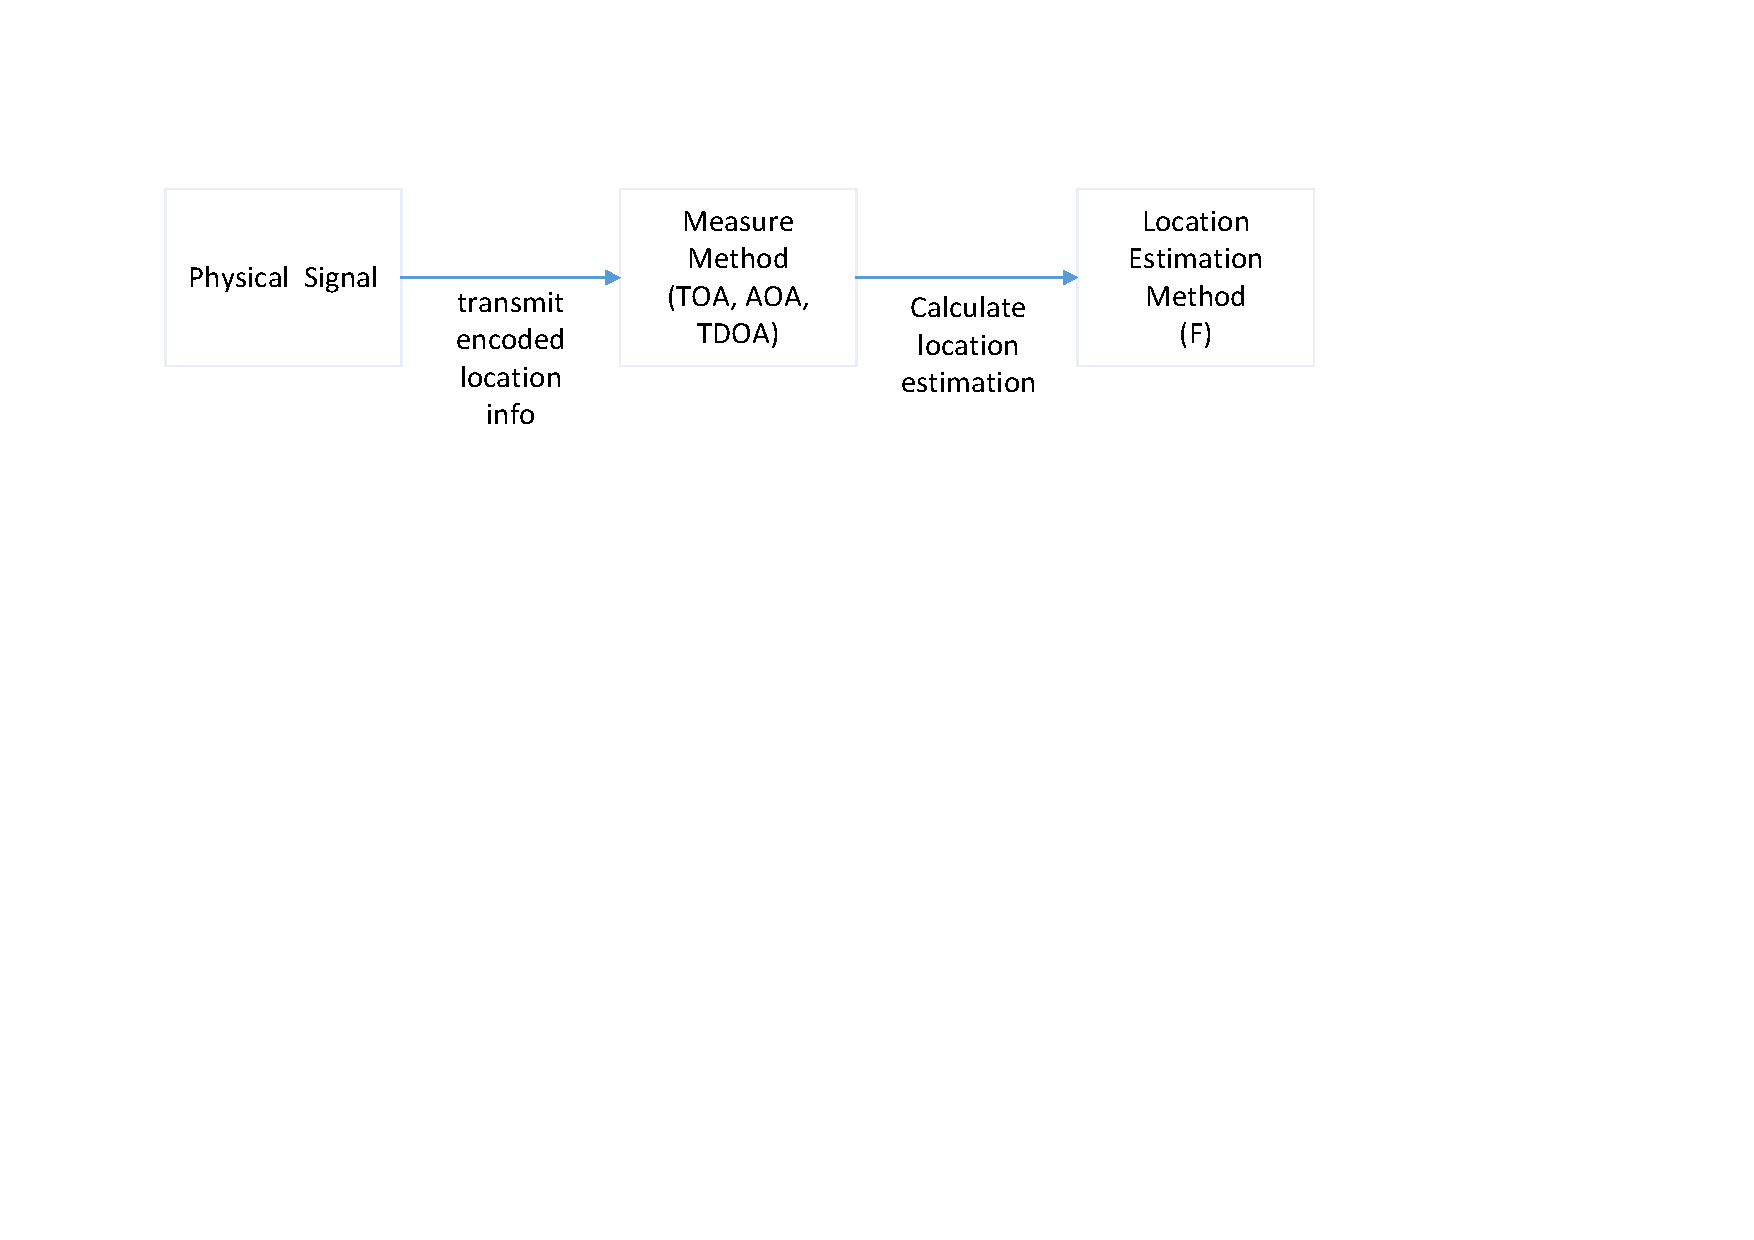
\includegraphics[width=3.5in]{../img.origin/fig1.pdf}
	\caption{Architecture of general IPS.}
	\label{fig_sim}
	\end{figure}

An indoor positioning system generally has an architecture of 3 phrases as shown in Figure 1. First step is to expose physical signals that contains the location information by US, IR, RF or other signals described above. These signal travels between emitter and receiver token by users. Then various methods are applied to calculate the physical quantity like measuring time of flight(TOF), time of arrival (TOA), time different of arrival (TDOA), angle of arrival (AOA), received signal strength (RSS) etc. With the raw information of a physical quantity measured, various techniques and algorithms are used which transform raw data into usable position information. Techniques have been classified as triangulation/trilateration [9], minmax algorithm [10], maximum likelihood[11] and fingerprinting [12].


RF systems estimate user location by measuring different properties of RF signals. RF Received Signal Strength Information (RSSI) has been employed for many different location estimation systems [13]. Performance of RSSI based location systems is highly effected by errors in signal strength resulted from multipath fading, reflection shadowing, diffraction etc [7]. Most of RSSI based IPS are exploiting WLAN as the media for physical signal since its low cost and convenience such as RADAR [2]. It uses signal strength information gathered at multiple receiver
locations to triangulate the user’s coordinates. Triangulation is done using both empirically-determined and theoretically computed signal strength information. Because the drawbacks mentioned above on WLAN's multipath effect or so, it can only reach an estimation accuracy of 10 meters.

Ultrasonic based IPS provide fine-grained location with centimeter level accuracy and it have higher capacity of location to serve many users simultaneously. As the work of Cricket[5], it relies on TOF measurement of US signal calculated using velocity of sound and other signal combined such as RF signal. But unlike RF signals, velocity of sound in air does not remain constant and varies largely with environmental condition especially humidity and temperature [7]. For example, the speed of sound is:
	\begin{equation}
	v_{us} = 20.05 \sqrt{T} 
	\end{equation}
Which means for each kelvin at normal indoor environment, the deviation is close to 0.18\%, an untolerated error. Another challenge to US systems is offered by high levels of environmental US noise. If noise is non-persistent, erroneous location estimates are filtered by use of suitable algorithms but persistent noise sources degrade system performance. Despite these challenges. deploying a US based IPS means a lot more hardware deployment work is to be done, and the users must be equipped with US receiver to get the system worked. This inconvenience can not be ignored in large-scale popularization.

RFID as a widely applicated low-cost hardware is also been developed as an method in IPS. Compared as RF and US signals, all RF tags can be read despite extreme environmental factors, such as snow, fog, ice, paint, and other visually and environmentally challenging conditions with a remarkable reading speed of less than 100 milliseconds. LANDMARC [8] is a RFID based IPS. It develops an algorithm to reflect the relations of signal strengths by power levels and maps which power level corresponds to what distance with the method of TDOA, and it reached a result of 2 meter level deviation. However it also have some problems. Currently available RFID products provides the signal strength of tags directly. Instead, the reader reports “detectable” or “not detectable” in a given range. This forces LANDMARC to spend approximately one minute each time to scan the 8 discrete power levels and to estimate the signal strength of tags which means the cost is unignorable. Besides, to apply this IPS, the mall needs to deploy several RFID tags and one RFID reader at an office-size area.

Apart from signal based IPS, there are works that relies on visible light to deliver the physical location information. Visible light are free of multipath, shadowing or attenuation of wireless signals, and are free from the influences of environmental temperature and moisture. 
One visible light based IPS, Epsilon [6], uses LED beacons and a custom light sensor that plugs into a smartphone’s audio port, and sometimes requires users to perform gestures. The LEDs transmit data using BFSK and avoid persistent collisions by random channel hopping. The system offers half-meter accuracy. This system requires custom hardware on user's phone and the performance can be improved.
Luxapose [1] is another visible light based IPS which relies on the LED luminaries deployed on ceilings to deliver physical location information and exploits CMOS smart phone camera to do some image processing work to get the physical signals, and by AOA algorithm it estimates the location with an accuracy of several centimeters. However in this work, each LED luminary exploits blink frequency to transmit raw message, and exploit CMOS camera's rolling shutter effect to receive these raw message in token pictures, which means the camera on smart phones must support sufficient wide range of exposure time to receive distinct LED signal. In its FFT method of decode the rolling shutter image into encoded frequency and the experiment platform of Lumia 1020 camera, it can only support about 20 distinct led beacons with the exposure frequency of camera up to 16000 Hz and the necessarily barrier between distinct LED signals of 500 Hz, and this problem is crucial in deploying this IPS in practical indoor malls or airports. Another issue is that for each time the user want to track himself/herself, he/she must take out the phone and shoot a picture of the LED luminaries on the ceilings. Obviously for each time, locating oneself needs to take a picture is not a good kind of user experience and many applications based on the track of people such as automatically merchant recommendation can not be implemented under this IPS. 

Table 1 is the benchmark comparison between the 5 IPS mentioned above.
	\begin{table}[!hbp]
	\begin{tabular}{|c|c|c|c|c|c|}
		
		\hline
		param & RADAR & Cricket & LANDMARC & Epsilon & Luxapose
		
		% \hline
		% Reference & [2] & [5] & [8] & [6] & [1]
	\end{tabular}
	\caption{Comparison of several IPS}
	\end{table}
	


\section{System Architecture}
This system consists of RGBLED based visible light beacons, smartphone with camera and a processing server as shown in Fig 2.
	
	\begin{figure}
		\centering
		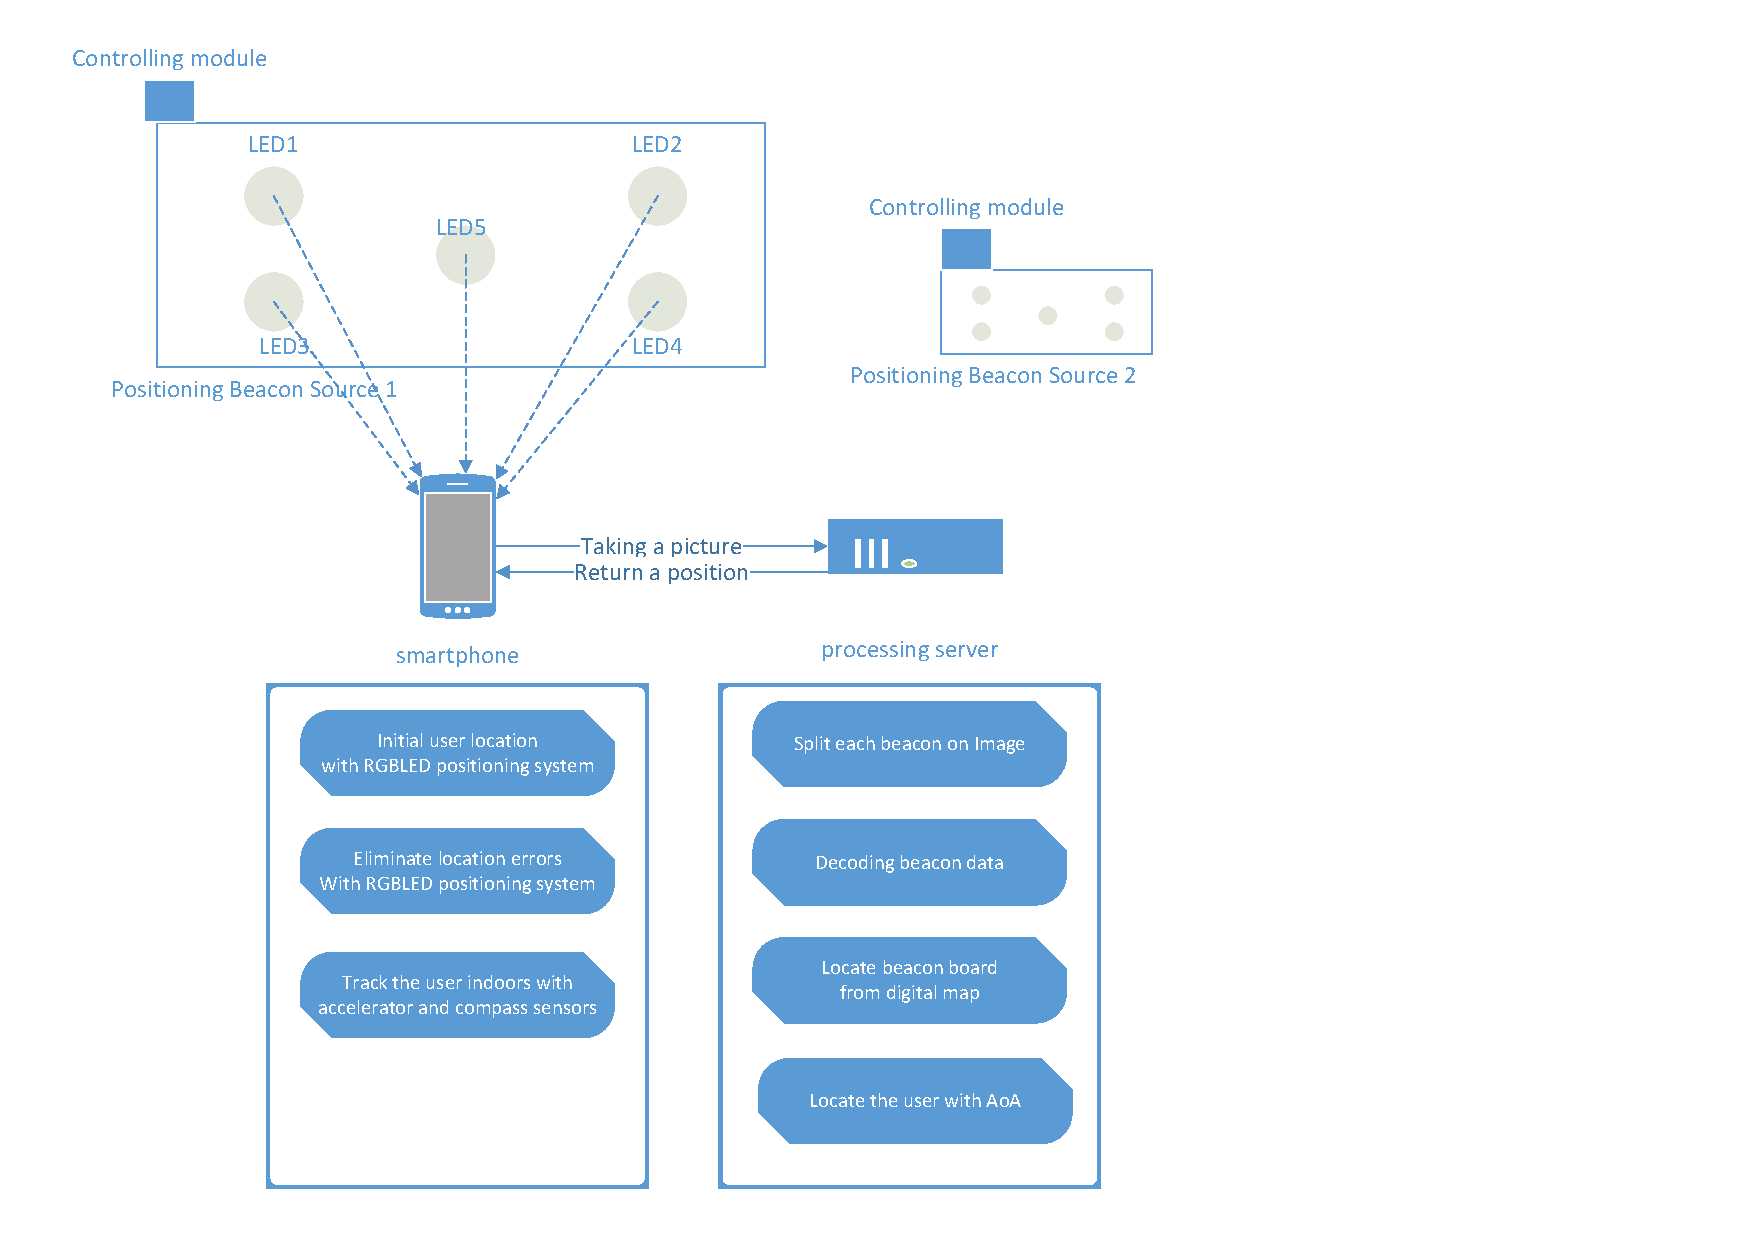
\includegraphics[width=3.5in]{../img.origin/fig2.pdf}
		\caption{Architecture of our system.}
		\label{fig_2}
	\end{figure}

We suppose an idea named \textbf{beacon source} as shown in the architecture Fig 2 of positioning beacon source 1 and positioning beacon source 2. In an indoor digital map, one distinct beacon source stands for one location coordinate on this map, and this coordinate is encoded in the light so if we can decode it we can roughly get our position nearby this coordinate. For each beacon source, the encoding data is provided by the controlling module which actually controls the flashing mechanism of each RGBLED bulb and we implemented it based on ArduinoDue board. In reality world, we can expolit the existing densely distributed RGBLED luminaries on ceilings of mall with only a low-cost PCB controller attached to its power supply to deploy our positioning hardware.

For each beacon source, it consists of no less than three RGBLED luminaries to support the angle-of-arrival algorithm. With knowing the roughly location with the help of beacon source and digital map, we can apply AoA algorithm so that we can calculate a relatively precise location of the user. 

For each time the user wants to locate himself/herself, it is necessary to take a picture and post it to the remote server and get the location. Clearly it is not convenient. So we developed an extended smartphone application which works with 3D accelerator sensor and compass sensor which can roughly track the user's locus. The accumulated error can be erased by taking an RGBLED positioning action.
	

\section{Basic Design}
Our system adpots an RGB mixed visible light as a communication channel to deliver locationing data. The RGBLED luminaries work as the transmitter and the smartphone camera works as the receiver. The encoding section describes how we encode digital map information into light signal with red, green and blue subchannels. The decoding section describes how we recover the message from mixed visible light. The positioning algorithm gives out detailed equations of angle of arrival that how can we measure the location based on all kinds of data we get.

\subsection{Encoding}
We deploy five RGBLED luminaries with their relative geometry known to provide redundancy in case some of them cannot be decoded. In fact under ideal circumstances three RGBLED luminaries will make the system locate the user's 3D location [14]. In other systems such as Luxapose [1] which exploits frequency as the method to distinguish different beacons, the major problem in practice is that it would need enough large barrier between the different frequencies so that the different stripes from rolling shutter effect could be distinguishable against the error casued by the photoing procedure. 
We introduce a novel encoding schema based on RGBLED with the method of frequency-domain multiplexing. By encoding different messages distinctly on red, green and blue channel with manchester coding which has a duty ratio of 50\% at a high frequency such as 4000Hz in our experiment, the beam radiates as white to human eyes which means this light can be used as normal illumination indoors.

The three channels work at a same frequency. We select the red channel as the clock channel, which means the red led will be light and dark at a constraint frequency, and it can cut consequent time into fixed size small pieces. The green and blue leds will perform each single signal in each piece based on red channel. The green channel encodes the geographic information of the beacon source the LED belongs to. The blue channel encodes the identity information that can tell the LEDs on the same beacon source apart. Fig. 3 shows one optional encoding implement with a coding length of 8 bit. The encoding digit length is restraint to how many stripes can be discovered on one single light spot on image, and this depends on the distance between camera and RED light as well as the resolution of camera. For our experiment case with Lumia 1020 camera, we can decode the image at a range up tp 5 meters with a resolution of 15M pixels, and under this circumstances we can encode in 8-dight length which stands for 8-bit symbol. So we can get $256 \times 256$ distinct RGBLED luminary. 

	\begin{figure}
		\centering
		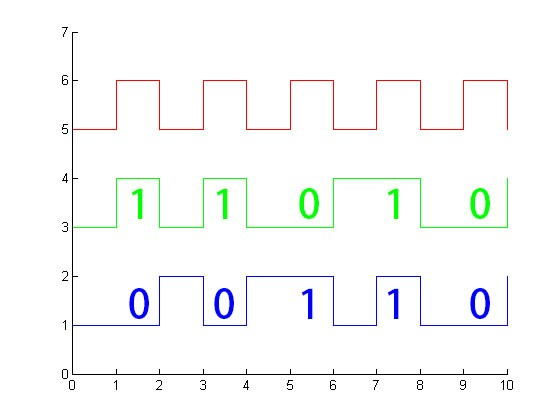
\includegraphics[width=3.5in]{../img.origin/fig3.jpg}
		\caption{Timing Diagram of Manchester Encoding.}
		\label{fig_3}
	\end{figure}

\subsection{Decoding}
First we need to find the centroid and size of each led spot on the rolling shutter image taken by the smartphone camera. The method is an image processing pipeline. First we need to rotate the picture to a standard manner since people take pictures in different angles. Then we convert the image to grayscale and we apply blur to it. After that we exploits a OTSU filter to find the edges of different spots on the image. We locates contours for different spots, and get the centroid by its circumcircle. With the centroid got, we know the spot maps to where on the image, and with the mask by the contour, we can respectively get each light spot for further processing. 

We need to calculate the encoding frequency with the help of rolling shutter effect. We can compress the image subregion of light spot vertical to the rolling shutter stripes, and outcome a vector and take an FFT of it. By this way we can convert the time-domain stripes into frequency-domain result with an error less than 200Hz. By declaring that the transmit frequency be interger multiplies of five hundred, we can enlarge the channel up to $n/1000$ times with $n$ stands for the reciprocal of exposure time parameter of smartphone camera, about 1/10000 second up to normal phones. For a smartphone with a camera of 1/10000 second exposure time, the expanding multiples of encoding channel is 10.  

In our encoding schema, for each timeslice, we can get a RGB value in one of the eight circumstances of {\#000000, \#0000ff, \#00ff00, \#00ffff, \#ff0000, \#ff00ff, \#ffff00, \#ffffff,}. The control unit can make it sure that each signal is strictly aligned in each timeslice. So the main idea is masking pure red to get timeslice gaps, and with the help of timeslice gaps, we use green and blue masks respectively to gain raw encoding information. 

\subsection{Positioning Algorithm}
By decoding the green channel with the aid from server end digital map data, we can roughly locate ourselves around one certain beacon source. We adopt the arrival of angle algorithm to obtain precious positioning results. With a well-token image which means at least three distinct RGBLED luminaries can be decodable, we can determine the 3D position of the camera with respect to the beacon source.

	\begin{figure}
		\centering
		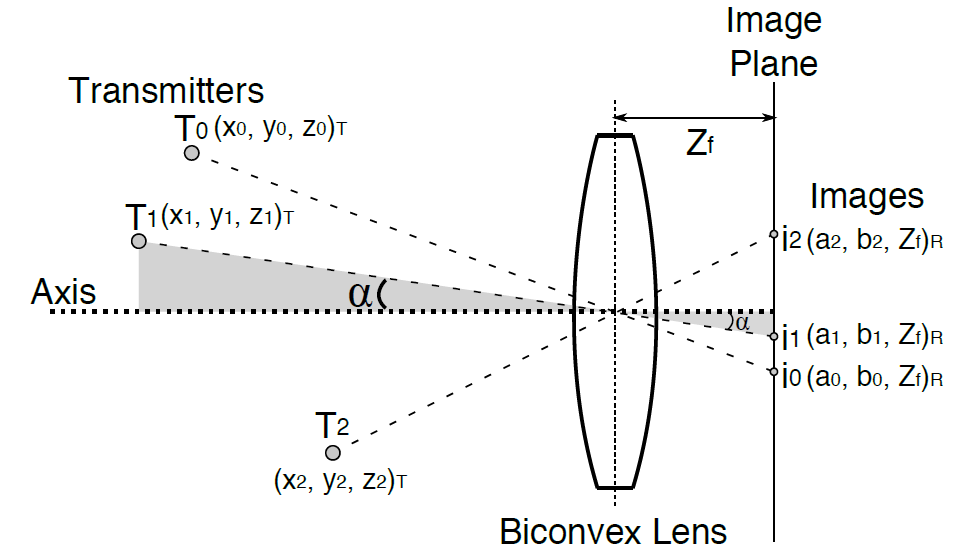
\includegraphics[width=3.5in]{../img.origin/fig4.png}
		\caption{AOA algorithm.}
		\label{fig_4}
	\end{figure}

As shown in Fig.4, the RGBLED luminary locate at point $T_0(x_0,y_0,z_0)_T$, this coordination is in the coordinate system on the positioning beacon source board and this is known to us but not the required coordination that we want to know. The luminary $T_0$ with the center of convex lens $(0,0,0)$ as well as the projection on the camera film $i_0(a_0, b_0, Z_f)_R$ stand in a line. $Z_f$ is the distance between lens and film, and $a_0$, $b_0$ can be got by locating the spot on the image as we talked above in section 4.2. Obvirously with geometry laws we can get the coordination of $T_0(u_0,v_0,w_0)$ that relative to the lens:
	\begin{equation}
	\begin{split}
	& 	u_0 = K_0 \times a_0\\	
	&	v_0 = K_0 \times b_0\\
	&	w_0 = K_0 \times Z_f
	\end{split}
	\end{equation}
Here $K_0$ is an unknown. Obvirously, the goal is to calculate $T_0(u_0,v_0,w_0)$. We have three pairs of this equation for three LED luminaries. And we know the location of $T_0(x_0,y_0,z_0)_T$,  $T_1(x_1,y_1,z_1)_T$ and  $T_2(x_2,y_2,z_2)_T$. Since we know the precise deploying location of $T_0$, $T_1$ and $T_2$, we can thus obtain the precise location of the user.

We define $d_0$ as the distance between $T_0$ and $T_1$, we can get the equation below:
	\begin{equation}
	\begin{split}
		&d_0^2 = (u_0 - u_1)^2 + (v_0 - v_1)^2 + (w_0 - w_1)^2  \\
		& \quad   =(K_0a_0-K_1a_1)^2 + (K_0b_0-K_1b_1)^2 +(K_0c_0-K_1c_1)^2  \\
		& \quad   =K_0^2[\vec{O_{l_0}}]^2 + K_1^2[\vec{O_{l_1}}]^2 - 2K_0K_1(\vec{O_{l_0}}\vec{O_{l_1}})
	\end{split}
	\end{equation}
Here $\vec{O_{l_0}}$ and $\vec{O_{l_1}}$ stand for a vector begin from the center of convex lens and end at $i_0(a_0, b_0, Z_f)_R$ and $i_1(a_1, b_1, Z_f)_R$. $K_0$ and $K_1$ are unknown to us. This is only two of the three LEDs, and by exploiting all three LEDs we can get a ternary quadratic group which means we can solve $K_0$, $K_1$ and $K_2$ out. With $K_0$, we can get the location of C with the help of equation[2]. Similarly we can get $T_1(u_1,v_1,w_1)$ and $T_2(u_2,v_2,w_2)$. 

However, this is an ideal scenario. Actually, the procedure when we locate the spot on image to get the $i_0(a_0, b_0, Z_f)_R$, we may generate cumullative errors. In order to reduce the errors, we transform the known coordinates of $T_0(x_0,y_0,z_0)_T$,  $T_1(x_1,y_1,z_1)_T$ and  $T_2(x_2,y_2,z_2)_T$ into an optimization problem.
\section{Implementation}
\subsection{Encoded RGBLED Board}
\subsection{Decoding and Positioning Server}
\subsection{Smart Phone Tracker}

\section{Performance and Evaluation}






% conference papers do not normally have an appendix


% use section* for acknowledgment
% \section*{Acknowledgment}


% The authors would like to thank...





% trigger a \newpage just before the given reference
% number - used to balance the columns on the last page
% adjust value as needed - may need to be readjusted if
% the document is modified later
%\IEEEtriggeratref{8}
% The "triggered" command can be changed if desired:
%\IEEEtriggercmd{\enlargethispage{-5in}}

% references section

% can use a bibliography generated by BibTeX as a .bbl file
% BibTeX documentation can be easily obtained at:
% http://mirror.ctan.org/biblio/bibtex/contrib/doc/
% The IEEEtran BibTeX style support page is at:
% http://www.michaelshell.org/tex/ieeetran/bibtex/
%\bibliographystyle{IEEEtran}
% argument is your BibTeX string definitions and bibliography database(s)
%\bibliography{IEEEabrv,../bib/paper}
%
% <OR> manually copy in the resultant .bbl file
% set second argument of \begin to the number of references
% (used to reserve space for the reference number labels box)
\begin{thebibliography}{1}

\bibitem{1,luxapose}
Ye-Sheng Kuo, Pat Pannuto, Ko-Jen Hsiao and Prabal Dutta. Luxapose: Indoor positioning with mobile phones and visible light. In Proc. 20th annual international conference on Mobile computing and networking (Mobicom ’14)
Pages 299-302.

\bibitem{2,radar}
P. Bahl and V. N. Padmanabhan. RADAR: An in-building
RF-based user location and tracking system. In Proc. 19th
Annual Joint Conference of the IEEE Computer and
Communications Societies. (INFOCOM ’00), volume 2, 2000.

\bibitem{3,cmos}
C. Danakis, M. Afgani, G. Povey, I. Underwood, and H. Haas, Using a CMOS camera sensor for visible light
communication, in Proceedings of the IEEE Workshop on Optical and Wireless Communication (OWC), pp. 1244-
1248, 2012.

\bibitem{4,ips without pain}
K. Chintalapudi, A. Padmanabha Iyer, and V. N.
Padmanabhan. Indoor localization without the pain. In Proc.
of the 16th ACM Annual International Conference on Mobile
Computing and Networking (MobiCom ’10), 2010.

\bibitem{5,ultrasonic}
Nissanka Bodhi Priyantha, Hari Balakrishnan, Erik Demaine, Seth Teller, Mobile-Assisted Localization in Wireless Sensor Networks, Proc. IEEE INFOCOM Conference, March 2005.

\bibitem{6,epsilon}
Liqun Li, Pan Hu, Guobin Shen, Chunyi Peng, Feng Zhao, Epsilon: A Visible Light Based Positioning System, the 11th USENIX Symposium on Networked Systems Design and Implementation, Seattle, Washington, 2014.

\bibitem{7,ultrasonic review}
Faheem Ijaz, Hee Kwon Yang, Arbab Waheed Ahmad, Chankil Lee. Indoor positioning: A review of indoor ultrasonic positioning systems, Advanced Communication Technology (ICACT).


\bibitem{8,rfid}
LIONEL M. NI and YUNHAO LIU, LANDMARC: Indoor Location Sensing Using Active RFID, Pervasive Computing and Communications, 2003. (PerCom 2003).

\bibitem{9,triangulation}
J. Hightower, SpotON: An Indoor 3D Location Sensing Technology Based on RF
Signal Strength, in: Department of Computer Science and Engineering,
University of Washington, Seattle, WA, 2000.

\bibitem{10,minmax}
K. Langendoen, N. Reijers, Distributed localization in wireless sensor networks:
a quantitative comparison, Computer Networks 43 (2003) 499–518.

\bibitem{11,maximum likelyhood}
M. Sugano, T. Kawazoe, Y. Ohta, M. Murata, Indoor Localization System Using
RSSI Measurement of Wireless Sensor Network Based on ZigBee Standard, in:
The IASTED International Conference on Wireless Sensor Networks (WSN
2006) Banff, Canada, 2006.

\bibitem{12,figerprinting}
K. Kaemarungsi and P. Krishnamurthy, Properties of indoor
received signal strength for WLAN location fingerprinting, The First Annual InternatIOnal Conference on Mobtle and UbiqUitous
Systems: Networking and Services, 2004. MOBIQU1TOUS 2004.

\bibitem{13, rssi}
E. Lau, ENHANCED RSSI-BASED HIGH ACCURACY REALTIME USER LOCATION TRACKING SYSTEM FOR INDOOR AND OUTDOOR ENVIRONMENTS International Journal, vol. 1, no. 2, 2008. 

\bibitem{14, aoa}
Se-Hoon Yang, Hyun-Seung Kim, Three-Dimensional Visible Light Indoor Localization Using AOA and RSS With Multiple Optical Receivers, Journal of Lightwave Technology(Volume:32 ,  Issue:14),2480 - 2485.
\end{thebibliography}






% that's all folks
\end{document}


